% Options for packages loaded elsewhere
\PassOptionsToPackage{unicode}{hyperref}
\PassOptionsToPackage{hyphens}{url}
\PassOptionsToPackage{dvipsnames,svgnames,x11names}{xcolor}
%
\documentclass[
  letterpaper,
  DIV=11,
  numbers=noendperiod]{scrartcl}

\usepackage{amsmath,amssymb}
\usepackage{iftex}
\ifPDFTeX
  \usepackage[T1]{fontenc}
  \usepackage[utf8]{inputenc}
  \usepackage{textcomp} % provide euro and other symbols
\else % if luatex or xetex
  \usepackage{unicode-math}
  \defaultfontfeatures{Scale=MatchLowercase}
  \defaultfontfeatures[\rmfamily]{Ligatures=TeX,Scale=1}
\fi
\usepackage{lmodern}
\ifPDFTeX\else  
    % xetex/luatex font selection
\fi
% Use upquote if available, for straight quotes in verbatim environments
\IfFileExists{upquote.sty}{\usepackage{upquote}}{}
\IfFileExists{microtype.sty}{% use microtype if available
  \usepackage[]{microtype}
  \UseMicrotypeSet[protrusion]{basicmath} % disable protrusion for tt fonts
}{}
\makeatletter
\@ifundefined{KOMAClassName}{% if non-KOMA class
  \IfFileExists{parskip.sty}{%
    \usepackage{parskip}
  }{% else
    \setlength{\parindent}{0pt}
    \setlength{\parskip}{6pt plus 2pt minus 1pt}}
}{% if KOMA class
  \KOMAoptions{parskip=half}}
\makeatother
\usepackage{xcolor}
\setlength{\emergencystretch}{3em} % prevent overfull lines
\setcounter{secnumdepth}{-\maxdimen} % remove section numbering
% Make \paragraph and \subparagraph free-standing
\makeatletter
\ifx\paragraph\undefined\else
  \let\oldparagraph\paragraph
  \renewcommand{\paragraph}{
    \@ifstar
      \xxxParagraphStar
      \xxxParagraphNoStar
  }
  \newcommand{\xxxParagraphStar}[1]{\oldparagraph*{#1}\mbox{}}
  \newcommand{\xxxParagraphNoStar}[1]{\oldparagraph{#1}\mbox{}}
\fi
\ifx\subparagraph\undefined\else
  \let\oldsubparagraph\subparagraph
  \renewcommand{\subparagraph}{
    \@ifstar
      \xxxSubParagraphStar
      \xxxSubParagraphNoStar
  }
  \newcommand{\xxxSubParagraphStar}[1]{\oldsubparagraph*{#1}\mbox{}}
  \newcommand{\xxxSubParagraphNoStar}[1]{\oldsubparagraph{#1}\mbox{}}
\fi
\makeatother

\usepackage{color}
\usepackage{fancyvrb}
\newcommand{\VerbBar}{|}
\newcommand{\VERB}{\Verb[commandchars=\\\{\}]}
\DefineVerbatimEnvironment{Highlighting}{Verbatim}{commandchars=\\\{\}}
% Add ',fontsize=\small' for more characters per line
\usepackage{framed}
\definecolor{shadecolor}{RGB}{241,243,245}
\newenvironment{Shaded}{\begin{snugshade}}{\end{snugshade}}
\newcommand{\AlertTok}[1]{\textcolor[rgb]{0.68,0.00,0.00}{#1}}
\newcommand{\AnnotationTok}[1]{\textcolor[rgb]{0.37,0.37,0.37}{#1}}
\newcommand{\AttributeTok}[1]{\textcolor[rgb]{0.40,0.45,0.13}{#1}}
\newcommand{\BaseNTok}[1]{\textcolor[rgb]{0.68,0.00,0.00}{#1}}
\newcommand{\BuiltInTok}[1]{\textcolor[rgb]{0.00,0.23,0.31}{#1}}
\newcommand{\CharTok}[1]{\textcolor[rgb]{0.13,0.47,0.30}{#1}}
\newcommand{\CommentTok}[1]{\textcolor[rgb]{0.37,0.37,0.37}{#1}}
\newcommand{\CommentVarTok}[1]{\textcolor[rgb]{0.37,0.37,0.37}{\textit{#1}}}
\newcommand{\ConstantTok}[1]{\textcolor[rgb]{0.56,0.35,0.01}{#1}}
\newcommand{\ControlFlowTok}[1]{\textcolor[rgb]{0.00,0.23,0.31}{\textbf{#1}}}
\newcommand{\DataTypeTok}[1]{\textcolor[rgb]{0.68,0.00,0.00}{#1}}
\newcommand{\DecValTok}[1]{\textcolor[rgb]{0.68,0.00,0.00}{#1}}
\newcommand{\DocumentationTok}[1]{\textcolor[rgb]{0.37,0.37,0.37}{\textit{#1}}}
\newcommand{\ErrorTok}[1]{\textcolor[rgb]{0.68,0.00,0.00}{#1}}
\newcommand{\ExtensionTok}[1]{\textcolor[rgb]{0.00,0.23,0.31}{#1}}
\newcommand{\FloatTok}[1]{\textcolor[rgb]{0.68,0.00,0.00}{#1}}
\newcommand{\FunctionTok}[1]{\textcolor[rgb]{0.28,0.35,0.67}{#1}}
\newcommand{\ImportTok}[1]{\textcolor[rgb]{0.00,0.46,0.62}{#1}}
\newcommand{\InformationTok}[1]{\textcolor[rgb]{0.37,0.37,0.37}{#1}}
\newcommand{\KeywordTok}[1]{\textcolor[rgb]{0.00,0.23,0.31}{\textbf{#1}}}
\newcommand{\NormalTok}[1]{\textcolor[rgb]{0.00,0.23,0.31}{#1}}
\newcommand{\OperatorTok}[1]{\textcolor[rgb]{0.37,0.37,0.37}{#1}}
\newcommand{\OtherTok}[1]{\textcolor[rgb]{0.00,0.23,0.31}{#1}}
\newcommand{\PreprocessorTok}[1]{\textcolor[rgb]{0.68,0.00,0.00}{#1}}
\newcommand{\RegionMarkerTok}[1]{\textcolor[rgb]{0.00,0.23,0.31}{#1}}
\newcommand{\SpecialCharTok}[1]{\textcolor[rgb]{0.37,0.37,0.37}{#1}}
\newcommand{\SpecialStringTok}[1]{\textcolor[rgb]{0.13,0.47,0.30}{#1}}
\newcommand{\StringTok}[1]{\textcolor[rgb]{0.13,0.47,0.30}{#1}}
\newcommand{\VariableTok}[1]{\textcolor[rgb]{0.07,0.07,0.07}{#1}}
\newcommand{\VerbatimStringTok}[1]{\textcolor[rgb]{0.13,0.47,0.30}{#1}}
\newcommand{\WarningTok}[1]{\textcolor[rgb]{0.37,0.37,0.37}{\textit{#1}}}

\providecommand{\tightlist}{%
  \setlength{\itemsep}{0pt}\setlength{\parskip}{0pt}}\usepackage{longtable,booktabs,array}
\usepackage{calc} % for calculating minipage widths
% Correct order of tables after \paragraph or \subparagraph
\usepackage{etoolbox}
\makeatletter
\patchcmd\longtable{\par}{\if@noskipsec\mbox{}\fi\par}{}{}
\makeatother
% Allow footnotes in longtable head/foot
\IfFileExists{footnotehyper.sty}{\usepackage{footnotehyper}}{\usepackage{footnote}}
\makesavenoteenv{longtable}
\usepackage{graphicx}
\makeatletter
\newsavebox\pandoc@box
\newcommand*\pandocbounded[1]{% scales image to fit in text height/width
  \sbox\pandoc@box{#1}%
  \Gscale@div\@tempa{\textheight}{\dimexpr\ht\pandoc@box+\dp\pandoc@box\relax}%
  \Gscale@div\@tempb{\linewidth}{\wd\pandoc@box}%
  \ifdim\@tempb\p@<\@tempa\p@\let\@tempa\@tempb\fi% select the smaller of both
  \ifdim\@tempa\p@<\p@\scalebox{\@tempa}{\usebox\pandoc@box}%
  \else\usebox{\pandoc@box}%
  \fi%
}
% Set default figure placement to htbp
\def\fps@figure{htbp}
\makeatother

\usepackage{float}
\usepackage{tabularray}
\usepackage[normalem]{ulem}
\usepackage{graphicx}
\UseTblrLibrary{booktabs}
\UseTblrLibrary{rotating}
\UseTblrLibrary{siunitx}
\NewTableCommand{\tinytableDefineColor}[3]{\definecolor{#1}{#2}{#3}}
\newcommand{\tinytableTabularrayUnderline}[1]{\underline{#1}}
\newcommand{\tinytableTabularrayStrikeout}[1]{\sout{#1}}
\usepackage{booktabs}
\usepackage{caption}
\usepackage{longtable}
\usepackage{colortbl}
\usepackage{array}
\usepackage{anyfontsize}
\usepackage{multirow}
\KOMAoption{captions}{tableheading}
\makeatletter
\@ifpackageloaded{caption}{}{\usepackage{caption}}
\AtBeginDocument{%
\ifdefined\contentsname
  \renewcommand*\contentsname{Table of contents}
\else
  \newcommand\contentsname{Table of contents}
\fi
\ifdefined\listfigurename
  \renewcommand*\listfigurename{List of Figures}
\else
  \newcommand\listfigurename{List of Figures}
\fi
\ifdefined\listtablename
  \renewcommand*\listtablename{List of Tables}
\else
  \newcommand\listtablename{List of Tables}
\fi
\ifdefined\figurename
  \renewcommand*\figurename{Figure}
\else
  \newcommand\figurename{Figure}
\fi
\ifdefined\tablename
  \renewcommand*\tablename{Table}
\else
  \newcommand\tablename{Table}
\fi
}
\@ifpackageloaded{float}{}{\usepackage{float}}
\floatstyle{ruled}
\@ifundefined{c@chapter}{\newfloat{codelisting}{h}{lop}}{\newfloat{codelisting}{h}{lop}[chapter]}
\floatname{codelisting}{Listing}
\newcommand*\listoflistings{\listof{codelisting}{List of Listings}}
\makeatother
\makeatletter
\makeatother
\makeatletter
\@ifpackageloaded{caption}{}{\usepackage{caption}}
\@ifpackageloaded{subcaption}{}{\usepackage{subcaption}}
\makeatother

\usepackage{bookmark}

\IfFileExists{xurl.sty}{\usepackage{xurl}}{} % add URL line breaks if available
\urlstyle{same} % disable monospaced font for URLs
\hypersetup{
  pdftitle={A Simulated DiD Analysis},
  colorlinks=true,
  linkcolor={blue},
  filecolor={Maroon},
  citecolor={Blue},
  urlcolor={Blue},
  pdfcreator={LaTeX via pandoc}}


\title{A Simulated DiD Analysis}
\author{}
\date{}

\begin{document}
\maketitle


\begin{Shaded}
\begin{Highlighting}[]
\FunctionTok{suppressWarnings}\NormalTok{(}\FunctionTok{suppressPackageStartupMessages}\NormalTok{(\{}
    \FunctionTok{library}\NormalTok{(modelsummary)}
    \FunctionTok{library}\NormalTok{(fixest)}
    \FunctionTok{library}\NormalTok{(gt)}
\NormalTok{\}))}
\FunctionTok{source}\NormalTok{(}\StringTok{"code/did\_sim\_utils.R"}\NormalTok{)}

\CommentTok{\# Ensure reproducibility by setting a seed for the random number generator}
\CommentTok{\# If you comment this out you will get a new random sample each call but}
\CommentTok{\# the results for the repeated simulation results will remain constant}
\CommentTok{\# as they are pre{-}run based on the seed set in \textasciigrave{}code/did\_sim\_create\_results.R\textasciigrave{}}

\FunctionTok{set.seed}\NormalTok{(}\DecValTok{04}\NormalTok{)}
\end{Highlighting}
\end{Shaded}

\subsubsection{The Simulated Data}\label{the-simulated-data}

We use a simulated sample inspired by
\href{https://doi.org/10.1093/rfs/hhn053}{Petersen (RFS, 2009)}. The
sample is based on 30 `countries'. Each country consists of 500 `firms'.
The panel is 10 `years' long.

We simulate a normally distributed outcome variable \(y\). For each firm
\(f\) in each country \(c\), the outcome variable for the first year
(\(y_{c,f,1}\)) is modeled to be

\(y_{c,f,1} = \gamma_c + \lambda_f + \psi_y + \varepsilon_{c,1} + \varepsilon_{f,1}\)

with
\(\gamma_c, \lambda_f, \psi_y, \varepsilon_{c,1}, \varepsilon_{f,1} \sim \sqrt{\frac{1}{5}}\mathcal{N}(0,1)\)

Meaning that in the first year, y is simply the sum of five normally
distributed random variables, weighted so that \(\sigma_y\) = 1. The
first three terms (\(gamma_c\), \(lambda_f\), and \(psi_y\)) represent
country, firm, and year fixed effects.

In the next period however, we model the country- and firm-level error
terms (\(\varepsilon_c\) and \(\varepsilon_f\)) both to autocorrelated
by the factors \(\rho_{c}\) and \(\rho_f\) so that

\(\varepsilon_{c,y} = \rho_{c}\varepsilon_{c,y-1} + \sqrt{1-\rho_{c}^2}\mathcal{N}(0,1)\)

and

\(\varepsilon_{f,y} = \rho_{f}\varepsilon_{f,y-1} + \sqrt{1-\rho_{f}^2}\mathcal{N}(0,1)\)

This implies that the dependent variable \(y\) is random but has

\begin{itemize}
\tightlist
\item
  stationary country-, firm- and time-level components and
\item
  an error term that is clustered by country and by firm.
\end{itemize}

\subsection{Injecting a Treatment
Effect}\label{injecting-a-treatment-effect}

We now pick half of the countries randomly. These countries are assumed
to receive treatment in year 6. We inject an effect size of 0.2. As
\(y\) has a baseline standard deviation of 1, this can be interpreted as
a small effect in Cohen's d terms.

Let's see how the data look by year and treatment group.

\begin{Shaded}
\begin{Highlighting}[]
\CommentTok{\# Take a look at the sim\_sample() function in \textasciigrave{}code/did\_sim\_utils.R\textasciigrave{} to learn}
\CommentTok{\# how we implemented the simulation in code.}

\NormalTok{smp }\OtherTok{\textless{}{-}} \FunctionTok{sim\_sample}\NormalTok{()}

\FunctionTok{ggplot}\NormalTok{(smp, }\FunctionTok{aes}\NormalTok{(}\AttributeTok{x =}\NormalTok{ year, }\AttributeTok{y =}\NormalTok{ y, }\AttributeTok{color =}\NormalTok{ treatment, }\AttributeTok{group =}\NormalTok{ treatment)) }\SpecialCharTok{+}
    \FunctionTok{geom\_pointrange}\NormalTok{(}
        \AttributeTok{stat =} \StringTok{"summary"}\NormalTok{,}
        \AttributeTok{fun =}\NormalTok{ mean, }
        \AttributeTok{fun.min =} \ControlFlowTok{function}\NormalTok{(x) }\FunctionTok{mean}\NormalTok{(x) }\SpecialCharTok{{-}} \FloatTok{1.96}\SpecialCharTok{*}\FunctionTok{sd}\NormalTok{(x)}\SpecialCharTok{/}\FunctionTok{sqrt}\NormalTok{(}\FunctionTok{length}\NormalTok{(x)), }
        \AttributeTok{fun.max =} \ControlFlowTok{function}\NormalTok{(x) }\FunctionTok{mean}\NormalTok{(x) }\SpecialCharTok{+} \FloatTok{1.96}\SpecialCharTok{*}\FunctionTok{sd}\NormalTok{(x)}\SpecialCharTok{/}\FunctionTok{sqrt}\NormalTok{(}\FunctionTok{length}\NormalTok{(x)) }
\NormalTok{    ) }\SpecialCharTok{+}
    \FunctionTok{scale\_x\_continuous}\NormalTok{(}\AttributeTok{breaks =} \DecValTok{1}\SpecialCharTok{:}\NormalTok{NYEARS) }\SpecialCharTok{+}
    \FunctionTok{labs}\NormalTok{(}\AttributeTok{x =} \StringTok{"Year"}\NormalTok{, }\AttributeTok{y =} \StringTok{"Y"}\NormalTok{, }\AttributeTok{color =} \StringTok{"Group"}\NormalTok{) }\SpecialCharTok{+}
    \FunctionTok{scale\_color\_discrete}\NormalTok{(}\AttributeTok{labels =} \FunctionTok{c}\NormalTok{(}\StringTok{"Control"}\NormalTok{, }\StringTok{"Treatment"}\NormalTok{)) }\SpecialCharTok{+} 
    \FunctionTok{theme\_minimal}\NormalTok{() }\SpecialCharTok{+}
    \FunctionTok{theme}\NormalTok{(}\AttributeTok{panel.grid.minor =} \FunctionTok{element\_blank}\NormalTok{())}
\end{Highlighting}
\end{Shaded}

\begin{center}
\pandocbounded{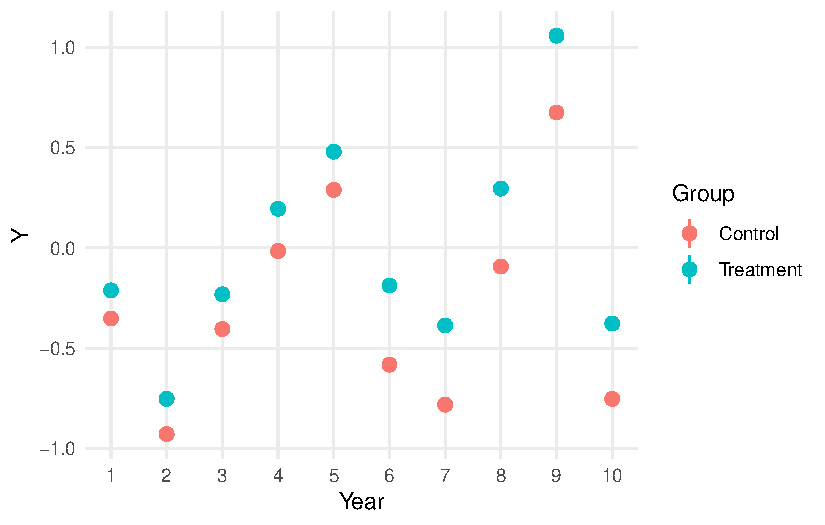
\includegraphics[keepaspectratio]{did_simulation_files/figure-pdf/unnamed-chunk-1-1.pdf}}
\end{center}

Wild, right? This is mostly because of the year fixed effects
\(\psi_y\). if you visualize the data using a typical event study plot,
everything looks much nicer.

\begin{Shaded}
\begin{Highlighting}[]
\NormalTok{est\_did }\OtherTok{\textless{}{-}} \FunctionTok{feols}\NormalTok{(y }\SpecialCharTok{\textasciitilde{}} \FunctionTok{i}\NormalTok{(year, treatment, }\DecValTok{5}\NormalTok{) }\SpecialCharTok{|}\NormalTok{ firm }\SpecialCharTok{+}\NormalTok{ year, smp)}
\FunctionTok{iplot}\NormalTok{(est\_did)}
\end{Highlighting}
\end{Shaded}

\begin{center}
\pandocbounded{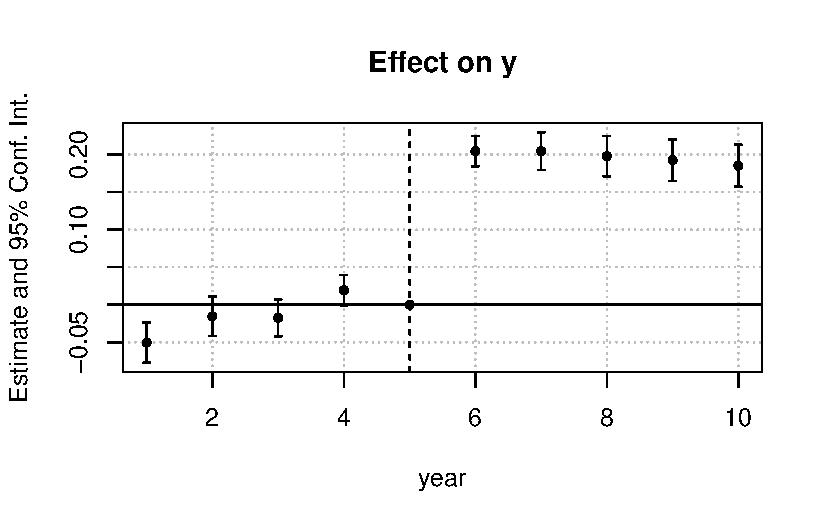
\includegraphics[keepaspectratio]{did_simulation_files/figure-pdf/unnamed-chunk-2-1.pdf}}
\end{center}

If these data were ``real'' they would look almost ``too good to be
true''.

\subsubsection{Comparing various
DiD-Models}\label{comparing-various-did-models}

Now we can compare the different types of estimators for this simulated
sample. We will compare the following estimation methods:

\begin{itemize}
\tightlist
\item
  A standard difference-in-differences estimator (pooling the pre and
  post-treatment observations)
\item
  A two-way fixed effects difference-in-differences estimator with
  various standard error clustering: none, by firm, by
  country\footnote{We do not need and should not use two-way clustering
    here as our clusters are nested (each firm belongs to one and only
    one country).}
\end{itemize}

\begin{Shaded}
\begin{Highlighting}[]
\NormalTok{mods }\OtherTok{\textless{}{-}} \FunctionTok{est\_models}\NormalTok{(smp)}
\NormalTok{mstats }\OtherTok{\textless{}{-}} \FunctionTok{create\_stats}\NormalTok{(mods)}

\FunctionTok{names}\NormalTok{(mods) }\OtherTok{\textless{}{-}} \FunctionTok{c}\NormalTok{(}\StringTok{"Standard DiD"}\NormalTok{, }\FunctionTok{rep}\NormalTok{(}\StringTok{"Two{-}Way FE"}\NormalTok{, }\DecValTok{3}\NormalTok{))}
\NormalTok{my\_fmt }\OtherTok{\textless{}{-}} \ControlFlowTok{function}\NormalTok{(x, }\AttributeTok{format =} \StringTok{"f"}\NormalTok{, }\AttributeTok{digits =} \DecValTok{3}\NormalTok{) }\FunctionTok{formatC}\NormalTok{(}
    \FunctionTok{as.numeric}\NormalTok{(x), }\AttributeTok{format =}\NormalTok{ format, }\AttributeTok{digits =}\NormalTok{ digits, }\AttributeTok{big.mark=}\StringTok{","}
\NormalTok{)}
\FunctionTok{modelsummary}\NormalTok{(}
\NormalTok{    mods,}
    \AttributeTok{fmt =}\NormalTok{ my\_fmt, }
    \AttributeTok{estimate =} \StringTok{"\{estimate\}\{stars\}"}\NormalTok{,}
    \AttributeTok{stars =} \FunctionTok{c}\NormalTok{(}\StringTok{\textasciigrave{}}\AttributeTok{***}\StringTok{\textasciigrave{}} \OtherTok{=} \FloatTok{0.01}\NormalTok{, }\StringTok{\textasciigrave{}}\AttributeTok{**}\StringTok{\textasciigrave{}} \OtherTok{=} \FloatTok{0.05}\NormalTok{, }\StringTok{\textasciigrave{}}\AttributeTok{*}\StringTok{\textasciigrave{}} \OtherTok{=} \FloatTok{0.10}\NormalTok{),}
    \AttributeTok{coef\_map =} \FunctionTok{c}\NormalTok{(}
        \StringTok{"postTRUE"} \OtherTok{=} \StringTok{"post"}\NormalTok{,}
        \StringTok{"treatmentTRUE"} \OtherTok{=} \StringTok{"treatment"}\NormalTok{, }
        \StringTok{"postTRUE:treatmentTRUE"} \OtherTok{=} \StringTok{"post × treatment"}\NormalTok{, }
        \StringTok{"treatedTRUE"} \OtherTok{=} \StringTok{"treated"}
\NormalTok{    ),}
    \AttributeTok{gof\_map =} \FunctionTok{list}\NormalTok{(}
        \FunctionTok{list}\NormalTok{(}\AttributeTok{raw =} \StringTok{"FE:firm"}\NormalTok{, }\AttributeTok{clean =} \StringTok{"FE: firm"}\NormalTok{, }\AttributeTok{fmt =} \DecValTok{0}\NormalTok{),}
        \FunctionTok{list}\NormalTok{(}\AttributeTok{raw =} \StringTok{"FE:year"}\NormalTok{, }\AttributeTok{clean =} \StringTok{"FE: year"}\NormalTok{, }\AttributeTok{fmt =} \DecValTok{0}\NormalTok{),}
        \FunctionTok{list}\NormalTok{(}\AttributeTok{raw =} \StringTok{"vcov.type"}\NormalTok{, }\AttributeTok{clean =} \StringTok{"Clustering"}\NormalTok{, }\AttributeTok{fmt =} \DecValTok{0}\NormalTok{),}
        \FunctionTok{list}\NormalTok{(}\AttributeTok{raw =} \StringTok{"r.squared"}\NormalTok{, }\AttributeTok{clean =} \StringTok{"R{-}squared"}\NormalTok{, }\AttributeTok{fmt =} \DecValTok{3}\NormalTok{),}
        \FunctionTok{list}\NormalTok{(}\AttributeTok{raw =} \StringTok{"nobs"}\NormalTok{, }\AttributeTok{clean =} \StringTok{"Sample Size"}\NormalTok{, }\AttributeTok{fmt =} \DecValTok{0}\NormalTok{)}
\NormalTok{    )}
\NormalTok{)}
\end{Highlighting}
\end{Shaded}

\begin{verbatim}
Warning: 'xfun::attr()' is deprecated.
Use 'xfun::attr2()' instead.
See help("Deprecated")

Warning: 'xfun::attr()' is deprecated.
Use 'xfun::attr2()' instead.
See help("Deprecated")
\end{verbatim}

\begin{table}
\centering
\begin{tblr}[         %% tabularray outer open
]                     %% tabularray outer close
{                     %% tabularray inner open
colspec={Q[]Q[]Q[]Q[]Q[]},
column{2,3,4,5}={}{halign=c,},
column{1}={}{halign=l,},
hline{10}={1,2,3,4,5}{solid, black, 0.05em},
}                     %% tabularray inner close
\toprule
& Standard DiD & Two-Way FE & Two-Way FE  & Two-Way FE   \\ \midrule %% TinyTableHeader
post             & \num{-0.025}*** &                 &                 &                 \\
& (\num{0.007})   &                 &                 &                 \\
treatment        & \num{0.178}***  &                 &                 &                 \\
& (\num{0.007})   &                 &                 &                 \\
post × treatment & \num{0.210}***  &                 &                 &                 \\
& (\num{0.011})   &                 &                 &                 \\
treated          &                  & \num{0.210}*** & \num{0.210}*** & \num{0.210}*** \\
&                  & (\num{0.006})  & (\num{0.009})  & (\num{0.050})  \\
FE: firm         &                  & X               & X               & X               \\
FE: year         &                  & X               & X               & X               \\
Clustering       & IID              & IID             & by: firm        & by: country     \\
R-squared        & \num{0.023}     & \num{0.729}    & \num{0.729}    & \num{0.729}    \\
Sample Size      & \num{150000}    & \num{150000}   & \num{150000}   & \num{150000}   \\
\bottomrule
\end{tblr}
\end{table}

As you can see from the regression output, the DiD-estimators are the
same (0.21) across all models, but their standard errors vary across
specifications, with the one clustered by country being much larger than
the others.

\subsubsection{Findings from a Monte Carlo
Simulation}\label{findings-from-a-monte-carlo-simulation}

One advantage of simulating data generating processes is that we can
re-run the sample generation multiple times. With this
\href{https://en.wikipedia.org/wiki/Monte_Carlo_method}{Monte Carlo
Simulation}, we can verify whether the identical estimators were just
random luck and also get an idea about the correct standard error for
this specific data generating process.

So, let's do this exercise 1,000 times and compare the estimators from
the Standard DiD model with the ones from the two-way fixed effect
model.

\begin{Shaded}
\begin{Highlighting}[]
\CommentTok{\# I have prepped the simulation results by running }
\CommentTok{\# \textasciigrave{}code/did\_sim\_create\_results.R\textasciigrave{}}
\NormalTok{sim\_results }\OtherTok{\textless{}{-}} \FunctionTok{readRDS}\NormalTok{(}\StringTok{"data/generated/did\_sim\_results.rds"}\NormalTok{)}

\CommentTok{\# The different clustering only affects the model\textquotesingle{}s standard errors }
\CommentTok{\# and not the coefficient estimate so it suffices to compare the estimates}
\CommentTok{\# of the standard DiD with one two{-}way fixed effect variant,}
\FunctionTok{ggplot}\NormalTok{(}
    \FunctionTok{aes}\NormalTok{(}\AttributeTok{x =}\NormalTok{ est, }\AttributeTok{group =}\NormalTok{ model, }\AttributeTok{color =}\NormalTok{ model), }
    \AttributeTok{data =}\NormalTok{ sim\_results }\SpecialCharTok{\%\textgreater{}\%} \FunctionTok{filter}\NormalTok{(model }\SpecialCharTok{\%in\%} \FunctionTok{c}\NormalTok{(}\StringTok{"simple\_did"}\NormalTok{, }\StringTok{"twfe\_did\_iid"}\NormalTok{))}
\NormalTok{) }\SpecialCharTok{+}
    \FunctionTok{geom\_density}\NormalTok{() }\SpecialCharTok{+}
    \FunctionTok{scale\_color\_discrete}\NormalTok{(}\AttributeTok{labels =} \FunctionTok{c}\NormalTok{(}\StringTok{"Standard DiD"}\NormalTok{, }\StringTok{"Two{-}Way FE DiD"}\NormalTok{)) }\SpecialCharTok{+}
    \FunctionTok{labs}\NormalTok{(}\AttributeTok{x =} \StringTok{"Estimate"}\NormalTok{, }\AttributeTok{y =} \StringTok{"Density"}\NormalTok{, }\AttributeTok{color =} \StringTok{"Model type"}\NormalTok{) }\SpecialCharTok{+}
    \FunctionTok{theme\_minimal}\NormalTok{()}
\end{Highlighting}
\end{Shaded}

\begin{center}
\pandocbounded{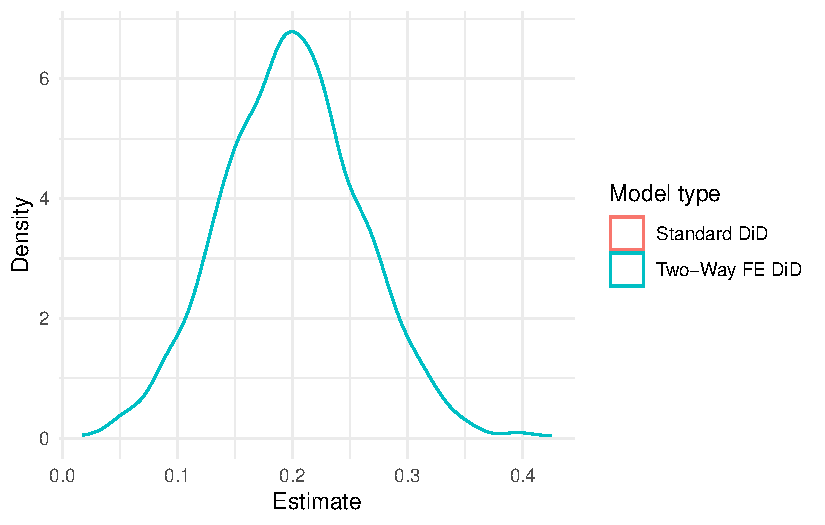
\includegraphics[keepaspectratio]{did_simulation_files/figure-pdf/unnamed-chunk-4-1.pdf}}
\end{center}

OK. The two estimator's density curves fully overlap, meaning that for
this well-specified data generating process, the standard DiD model
creates the same estimates as a two-way fixed effect model.

The standard deviation of our 1,000 estimators is 0.0602. This is close
to the standard error of the two-way fixed model with clustering by
country (0.0501) but much larger than the other standard errors,
e.g.~the one for the two-way fixed model with clustering by firm
(0.00867).

We can now assess whether the standard erros reported by the various
models are correct by comparing their averages to the actual standard
deviation of the estimator (0.0602). In addition, we can take a look at
the power of the models and their likelihood to generate Type I errors,
meaning to falsely produce significant findings.

\begin{Shaded}
\begin{Highlighting}[]
\NormalTok{sim\_result\_avgs }\OtherTok{\textless{}{-}}\NormalTok{ sim\_results }\SpecialCharTok{\%\textgreater{}\%} \FunctionTok{group\_by}\NormalTok{(model) }\SpecialCharTok{\%\textgreater{}\%} \FunctionTok{summarise}\NormalTok{(}
    \StringTok{\textasciigrave{}}\AttributeTok{Mean standard error}\StringTok{\textasciigrave{}} \OtherTok{=} \FunctionTok{mean}\NormalTok{(se),}
    \StringTok{\textasciigrave{}}\AttributeTok{Power of test (\%)}\StringTok{\textasciigrave{}} \OtherTok{=} \DecValTok{100} \SpecialCharTok{*} \FunctionTok{mean}\NormalTok{(lb }\SpecialCharTok{\textgreater{}} \DecValTok{0}\NormalTok{),}
    \StringTok{\textasciigrave{}}\AttributeTok{Type 1 Error (\%)}\StringTok{\textasciigrave{}} \OtherTok{=} \DecValTok{100} \SpecialCharTok{*} \FunctionTok{mean}\NormalTok{(lb }\SpecialCharTok{\textgreater{}}\NormalTok{ EFFECT\_SIZE }\SpecialCharTok{|}\NormalTok{ ub }\SpecialCharTok{\textless{}}\NormalTok{ EFFECT\_SIZE)}
\NormalTok{) }\SpecialCharTok{\%\textgreater{}\%} 
    \FunctionTok{ungroup}\NormalTok{() }\SpecialCharTok{\%\textgreater{}\%}
    \FunctionTok{mutate}\NormalTok{(}\AttributeTok{model =} \FunctionTok{factor}\NormalTok{(}
\NormalTok{        model, }
        \AttributeTok{levels =} \FunctionTok{c}\NormalTok{(}
            \StringTok{"simple\_did"}\NormalTok{, }\StringTok{"twfe\_did\_iid"}\NormalTok{, }
            \StringTok{"twfe\_did\_firm\_cl"}\NormalTok{, }\StringTok{"twfe\_did\_country\_cl"}
\NormalTok{        ),}
        \AttributeTok{labels =} \FunctionTok{c}\NormalTok{(}
            \StringTok{"Standard DiD"}\NormalTok{, }\StringTok{"TWFE DiD no clusters"}\NormalTok{, }
            \StringTok{"TWFE DiD firm clusters"}\NormalTok{, }\StringTok{"TWFE DiD country clusters"}
\NormalTok{        )}
\NormalTok{    )) }\SpecialCharTok{\%\textgreater{}\%}
    \FunctionTok{rename}\NormalTok{(}\AttributeTok{Model =}\NormalTok{ model) }\SpecialCharTok{\%\textgreater{}\%}
    \FunctionTok{arrange}\NormalTok{(Model)}

\NormalTok{sim\_result\_avgs }\SpecialCharTok{\%\textgreater{}\%} \FunctionTok{gt}\NormalTok{() }\SpecialCharTok{\%\textgreater{}\%} 
    \FunctionTok{fmt\_number}\NormalTok{(}\AttributeTok{columns =} \StringTok{\textasciigrave{}}\AttributeTok{Mean standard error}\StringTok{\textasciigrave{}}\NormalTok{, }\AttributeTok{decimals =} \DecValTok{3}\NormalTok{) }\SpecialCharTok{\%\textgreater{}\%}
    \FunctionTok{cols\_align}\NormalTok{(}\StringTok{"left"}\NormalTok{, Model)}
\end{Highlighting}
\end{Shaded}

\begin{table}
\fontsize{12.0pt}{14.4pt}\selectfont
\begin{tabular*}{\linewidth}{@{\extracolsep{\fill}}lrrr}
\toprule
Model & Mean standard error & Power of test (\%) & Type 1 Error (\%) \\ 
\midrule\addlinespace[2.5pt]
Standard DiD & 0.010 & 99.9 & 73.4 \\ 
TWFE DiD no clusters & 0.006 & 100.0 & 83.3 \\ 
TWFE DiD firm clusters & 0.009 & 100.0 & 75.7 \\ 
TWFE DiD country clusters & 0.060 & 88.9 & 4.9 \\ 
\bottomrule
\end{tabular*}
\end{table}

As you can see, only the standard errors generated by the two-way fixed
effect model with country-level clustering are correct in the sense that
they match the actual distribution of the simulated estimates. The other
standard errors are too narrow. This causes the other models to generate
95\% confidence intervals that often do not include the true effect of
0.2 (Type 1 Error). Only for country-level clustering this error rate is
about 5\% as it should be.

Finally, let's take a look at power. Power is the likelihood that the
model generates an estimate that is significantly different from zero.
It is foremost determined by the effect size that we simulate or expect
in real data. Here, we expect a relatively small effect size. Next,
power dependends on the size of the used sample. Here, we are using a
massive sample (30 countries times 500 firms times 10 years = 150,000
observations). Larger samples reduce standard errors, yielding more
power. Finally, clustering implies that standard errors are essentially
estimated at the cluster level. This means that the power of the
analysis will be affected by the number of cluster units (30 in our
case). The more units you have, the better.

In our simulation you see that clustering by country reduces the power
from virtually 100\% to 88.9\%. Still not bad but remember that we have
a massive sample and a very clean data generating process. Real life
data will be messier and samples will be smaller, yielding much less
power.

\subsubsection{Next steps}\label{next-steps}

This concludes this little simulation exercise. If you want to explore
further and learn more, here are some topics to think about:

\begin{itemize}
\tightlist
\item
  How would a variant of a Standard DiD model that uses country-level
  clusters perform?
\item
  When you vary the effect size how do you expect power to react? When
  will it fall below the often required power hurdle of 80\%?
\item
  What happens when you change sample parameters, e.g.~decrease the
  number of countries or number of firms per countries? Which parameter
  do you expect to be more influential for confidence intervals and
  power?
\end{itemize}




\end{document}
